A complete visualization of the tech stack can be found in \ref{fig:tech-stack}. Further details and explanations can be found in the following sections.

\begin{figure}[H]
    \centering
    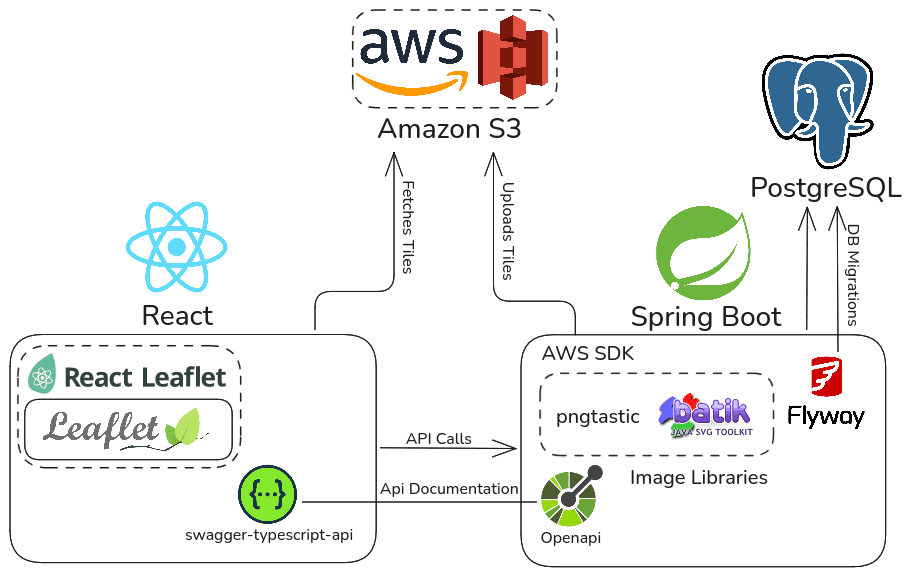
\includegraphics[scale=0.4]{pics/tech-stack.png}
    \caption{Tech Stack}
    \label{fig:tech-stack}
\end{figure}


\section{React}
\setauthor{Michael Ruep}
The frontend of SeatGen is built using the React framework. This choice was primarily motivated by the existing expertise within Solvistas, ensuring that the company’s developers could easily maintain and adjust the project to their needs. Additionally, React provides an ideal balance between flexibility, performance, and a vibrant ecosystem, which are factors that proved crucial when building an interactive seating plan editor for stadiums. Also, our team was already experienced with component-based single page application frontend frameworks.

\subsection{Framework Background}
React is an open-source JavaScript library developed and maintained by Meta (formerly known as Facebook) and a community of individual developers and companies. Originally introduced in 2013 to power Facebook’s dynamic news feed, React has since become renowned for creating data-driven web interfaces~\cite{ReactDocs, SPAComp}. Rather than manually manipulating the Document Object Model (DOM), developers can simply declare how the interface should appear based on the underlying data. This declarative approach allows React to handle updates internally, ensuring smoother user interactions, which are especially beneficial for large or frequently changing data sets~\cite{ReactVirtualDOM, SPAComp}.

\subsection{Virtual DOM}
\setauthor{Michael Ruep}
React’s Virtual DOM architecture is particularly advantageous for applications requiring frequent updates and complex UI interactions. In SeatGen, each seat on the map can be added, moved, or deleted in real time, causing rapid changes that must be reflected in the user interface without compromising speed. By selectively re-rendering only components that have actually changed, the Virtual DOM mechanism helps maintain excellent performance even under heavy load~\cite{ReactVirtualDOM}. This aligns with the findings in~\cite{SPAComp}, where React demonstrates superior rendering speed and user satisfaction in Single Page Applications (SPAs) requiring dynamic content updates.

\subsection{Component-based Architecture}
\setauthor{Michael Ruep}
React’s component-based architecture keeps each feature modular to make the project easier to maintain as it grows. Instead of bundling all functionality into a single monolithic view, UI features are developed as self-contained components. In our case for example:
\begin{compactitem}
    \item Seat Map Component
    \item Toolbar Component
    \item Detail Component
\end{compactitem}
Each of those elements has its own component, allowing developers to modify or expand individual features without affecting unrelated parts of the application. This approach simplifies debugging, since issues can often be traced to a specific component rather than across the entire codebase. It is also suitable for collaborative development by letting team members work on separate components in parallel, which significantly accelerated our development process. Overall, React’s modular design reduces complexity which assists a more organized and maintainable codebase.
~\cite{ReactCBA01, ReactCBA02, ReactCBA03}

\subsection{Integration of Libraries}
\setauthor{Michael Ruep}
One of SeatGen’s central requirements is to enable direct manipulation for seat layouts. React’s flexible architecture allows for the easy incorporation of third-party libraries. For example, Leaflet was integrated to render the stadium map using its efficient, canvas-based engine. React uses its Context API to manage global state and user interactions, while Leaflet is responsible for the map rendering. This separation ensures that intensive mapping operations do not interfere with overall UI responsiveness. Reacts Context was used to manage global state effectively. This approach meets the specific requirements of seat manipulation, multi-layered zoom levels, and user interactions.

\subsection{Developer Familiarity and Team Expertise}
\setauthor{Michael Ruep}
Since React was already in use at Solvistas, its adoption ensured that the company’s developers could seamlessly work with and extend the project. Additionally, our team had prior experience with component-based frontend frameworks, making it easy to understand React’s structure, including concepts such as routing, state management, data binding, and components. This familiarity enabled a quick understanding and utilization of React, leading to the rapid development of the first running prototype.

\subsubsection{Comparison to Other Frameworks}
\setauthor{Michael Ruep}
Compared to alternative frameworks such as Angular or Vue studies have shown that React and Vue generally demonstrate superior rendering performance and faster load times in dynamic applications~\cite{SPAComp}. Additionally, React is preferred by developers for SPAs with frequent UI updates, with a reported 34\% higher satisfaction rate compared to other frameworks~\cite{SPAComp}. 

\subsection{Summary}
\setauthor{Michael Ruep}
React’s widespread adoption, strong ecosystem, and proven efficiency in building dynamic web applications make it a reliable choice for modern frontend development. Its Virtual DOM ensures optimized rendering performance, while its component-based architecture keeps the application modular and maintainable. Additionally, React Context provides a lightweight yet effective solution for managing global state. This allows seamless integration with external libraries such as Leaflet for real-time seat rendering~\cite{ReactVirtualDOM, ReactCBA01}. 

With React already in use within the company, adopting it ensured maintainability and smooth collaboration. Its performance advantages in Single Page Applications (SPAs), along with high developer satisfaction rates~\cite{SPAComp}, further validated its suitability for our interactive seating plan editor.

\section{Leaflet}
\setauthor{Michael Ruep}
Leaflet is an open-source JavaScript library designed for interactive maps. Developed by Vladimir Agafonkin and maintained by a large community, it is widely used for its lightweight nature and ease of integration with modern web applications~\cite{Leaflet}. Unlike heavyweight mapping solutions such as Google Maps or OpenLayers, Leaflet is specifically optimized for rendering custom vector layers and handling dynamic user interactions efficiently. These characteristics make it an ideal choice for SeatGen’s stadium seat visualization, where real-time updates and performance optimization are critical.

\subsection{Reasons for Leaflet}
\setauthor{Michael Ruep}
For SeatGen, choosing the right mapping library was crucial to ensuring smooth and interactive seat visualization. Leaflet was selected due to its lightweight architecture, extensibility, and strong performance when rendering custom vector layers. Unlike Google Maps or OpenLayers, which offer extensive GIS (geographic information system focused) functionalities but often introduce unnecessary overhead, Leaflet is designed for fast, customizable, and lightweight mapping solutions~\cite{Leaflet}. 

A key advantage of Leaflet is its low dependency footprint. Unlike other mapping solutions that rely on external APIs or heavy SDKs, Leaflet provides a standalone JavaScript library that integrates seamlessly with React. This lightweight approach ensures excellent map performance, even when handling large stadiums with thousands of seats. In contrast, frameworks like Google Maps API enforce rate limits and external API calls, which can introduce latency and unnecessary costs.

Leaflet’s customizability also played a significant role in our decision. SeatGen requires custom zoom levels, and real-time updates, all of which are efficiently handled using Leaflet’s open architecture. Unlike proprietary mapping tools, Leaflet allows full control over rendering logic, making it easier to optimize performance and adjust the visualization to match stadium layouts precisely~\cite{Leaflet}. Furthermore, existing Leaflet functions were adapted for tasks such as seat selection and the grid tool. This significantly accelerated the development process

By selecting Leaflet, SeatGen ensures efficient handleing of multi-layered rendering, interactive zoom, custom maps, and seamless seat selection, all while maintaining a lightweight and scalable frontend architecture.

\subsection{Key Features Used in SeatGen}
\setauthor{Michael Ruep}

Leaflet provides several core functionalities that are essential for our interactive seating plan editor. The following features were particularly valuable in implementing a performant and user-friendly seat visualization system:

\begin{itemize}
    \item \textbf{Dynamic Seat Rendering:} Leaflet enables the efficient rendering of thousands of seat markers without significantly impacting performance. Since stadiums can contain a large number of seats, rendering was optimized using Leaflet layers to manage visibility at different zoom levels.
    \item \textbf{Custom Zoom Levels and Scaling:} Leaflet allows the definition of custom zoom levels, ensuring precise seat selection when zoomed in and a full view of the stadium’s structure when zoomed out.
    \item \textbf{Interactive Seat Selection:} By leveraging Leaflet’s built-in event handling system, users can click and modify seats in real time. This is crucial for intuitively adjusting seating arrangements.
    \item \textbf{Grid-Based Seat Placement:} Leaflet’s selection, polygon, and coordinate functions were used to implement functions like the grid tool and selection tool, allowing for structured seat placement. This feature speeds up the process of generating rows and sections by automatically aligning seats according to predefined parameters.
    \item \textbf{Real-Time State Management with React Context:} Since Leaflet does not natively integrate with React’s state management, React Context was used to synchronize seat selections, updates, and modifications across the application. This ensures that any seat change is reflected immediately in both the UI and the underlying data model.
\end{itemize}

These features collectively make Leaflet a powerful tool for handling the seat visualization requirements. By leveraging Leaflet’s efficient rendering engine and customization capabilities, a seamless user experience was created that allows for real-time adjustments and intuitive stadium navigation.

\subsection{Integration with React}
\setauthor{Michael Ruep}
Integrating Leaflet with React was straightforward thanks to React Leaflet, a library that provides React components for Leaflet~\cite{ReactLeafletDocs}. This greatly simplified the integration process, as Leaflet elements could be managed within React components without directly manipulating the DOM.

One challenge faced was handling state management and data binding between Leaflet and React. Since Leaflet operates independently of React’s Virtual DOM~\cite{ReactLeafletDocs}, synchronizing real-time seat selections, modifications, grid placements, and similar interactions required a structured approach.

Beyond standard Leaflet functionality, existing features were extended and customized to meet specific needs. Tools like the seat selection tool and grid tool leveraged Leaflet’s built-in functions but were adapted to suit SeatGen’s requirements. By understanding and modifying Leaflet’s core functions, a tailored solution was developed, aligning with the requirements for real-time seat arrangement and stadium visualization.

\subsection{Summary}
\setauthor{Michael Ruep}

Leaflet’s lightweight architecture, flexibility, and strong customization capabilities made it the ideal choice for an interactive seating plan editor. Unlike heavier GIS-focused alternatives, Leaflet provided a high-performance mapping solution tailored for real-time seat rendering and selection. 

Its custom zoom levels allowed for the creation of an intuitive and responsive seating visualization tool. Additionally, React Leaflet streamlined the integration process, enabling faster development within React~\cite{ReactLeafletDocs}.

By leveraging Leaflet’s existing functionality and extending its core features to suit stadium seat planning, a clean and efficient tool suite was ensured, enabling smooth real-time interaction. This solidifies Leaflet as an essential part of the frontend architecture.